\chapter[Introduction]{Introduction}
Chapter 1 will contain the introduction, the problem definition, the goal and objectives and in the end will explain the report-structure.

\section[Introduction]{Introduction}
\subsection{Challenges for an ageing population}
The Dutch population is getting older. In 2014, 18\% of the population was older than 65. In 2040 the demographic ageing will reach its top, 26\% of the population will be 65 years and older.~\cite{Hylkema2014} Amsterdam has less demographic ageing compared to the whole of Netherlands~\cite{Hylkema2014}. 22.4\% of its inhabitants is older than 55, in absolute numbers 182.000 inhabitants on 01-01-2014. See figure~\ref{demo}. One fifth of these elderly is older than 75 and 13\% older than 80.~\cite{Hylkema2014} By 2040, Amsterdam will have 11 to 16 percent more elderly inhabitants of above the age of 65. 

\begin{figure}[h]
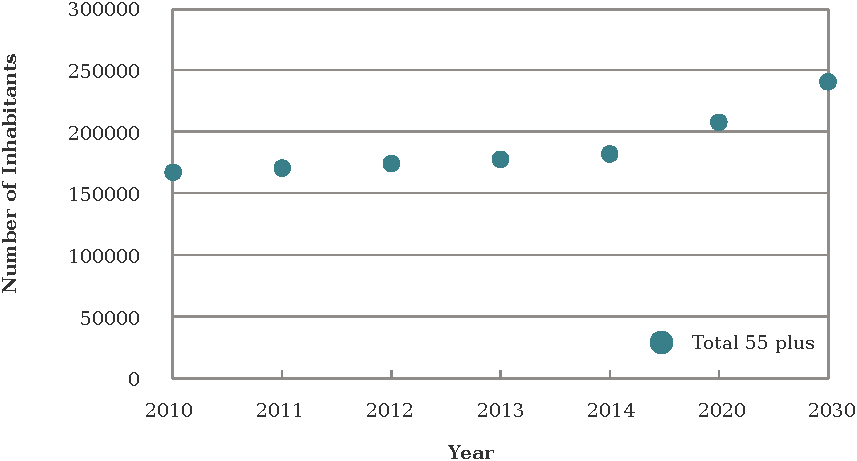
\includegraphics[width=\textwidth]{img/I1_number_elderly.pdf}
\centering
\caption[Total 55 plus inhabitants Amsterdam.]{
Total 55 plus inhabitants Amsterdam. On the 1st of January 2010-2014 \& Prognosis (2013) for 2020 and 2030. (Hylkema et al. 2014)} 
\label{demo}
\end{figure} 

Since 2015 the Dutch municipalities are responsible for the care of elderly, the assistance and support. The growing share of elderly is expected to demand higher funds regarding health care, social care and retirements wages but fewer funds are available for decentralized governments to spend on health care. These developments challenge to seek solutions to balance cost and services. Synergizing policy solutions between different policy areas at a decentralized level may help with the solution.~\cite{Hylkema2014} 

The new trend in elderly care is letting elderly live longer independently~\cite{MENSenSTRAAT2014, VandeRidder2008} also called active ageing~\cite{Annear2014}. The Amsterdam municipality aims its elderly strategy in the StructuurVisie for 2040 to let older inhabitants live independently, as long as possible, to reduce health care costs. Growing old in the own house, is welcomed by a lot of older inhabitants of Amsterdam.~\cite{Bossink2011}

\subsection{Elderly pedestrians}
Living independently means being mobile for personal care and have access to the public space for grocery shopping, social contacts and physical activity. In urban areas, elderly depend on walking for their everyday life and it is a key aspect of daily life to stay independent.~\cite{OECD2001}. Walking as form of transport happens more in urban areas then in rural(figure~\ref{walktrip}).
In many countries 30 to 50\% of older people's journeys outside are made as a pedestrian~\cite{Stahl2013}. In the Netherlands about 23\% of the trips made by elderly are made by foot. In Amsterdam 31\% of the main trips are made by foot. In general, Dutch elderly depend more on walking then other age groups as seen in figure \ref{percwalk} from a pedestrian study by CROW(explained in section 1.2.1).~\cite{Eijnde2011, Sauter2010, Crow2014}

\begin{figure}[h]
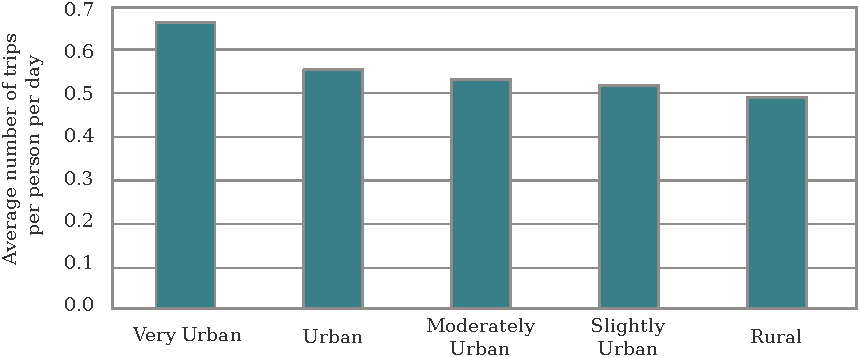
\includegraphics[width=\textwidth]{img/I2_urbanwalks.pdf}
\centering
\caption[Walking trips made in specific environment.]{Walking trips made in specific environment. (Sauter et al. 2010)
\label{walktrip}} 
\end{figure}

The main benefit of walking is the importance for the health of elderly.~\cite{Borst2008} Regular exercise has a positive effect on the fitness and physical health. Also lowering stress and improves the overall well-being. There is a well-established correlation between health benefits and regular physical activity.~\cite{Annear2014} Also, for elderly walking is the favoured form of physical activity.~\cite{Borst2008} See figure~\ref{percwalk}.

\begin{figure}[h]
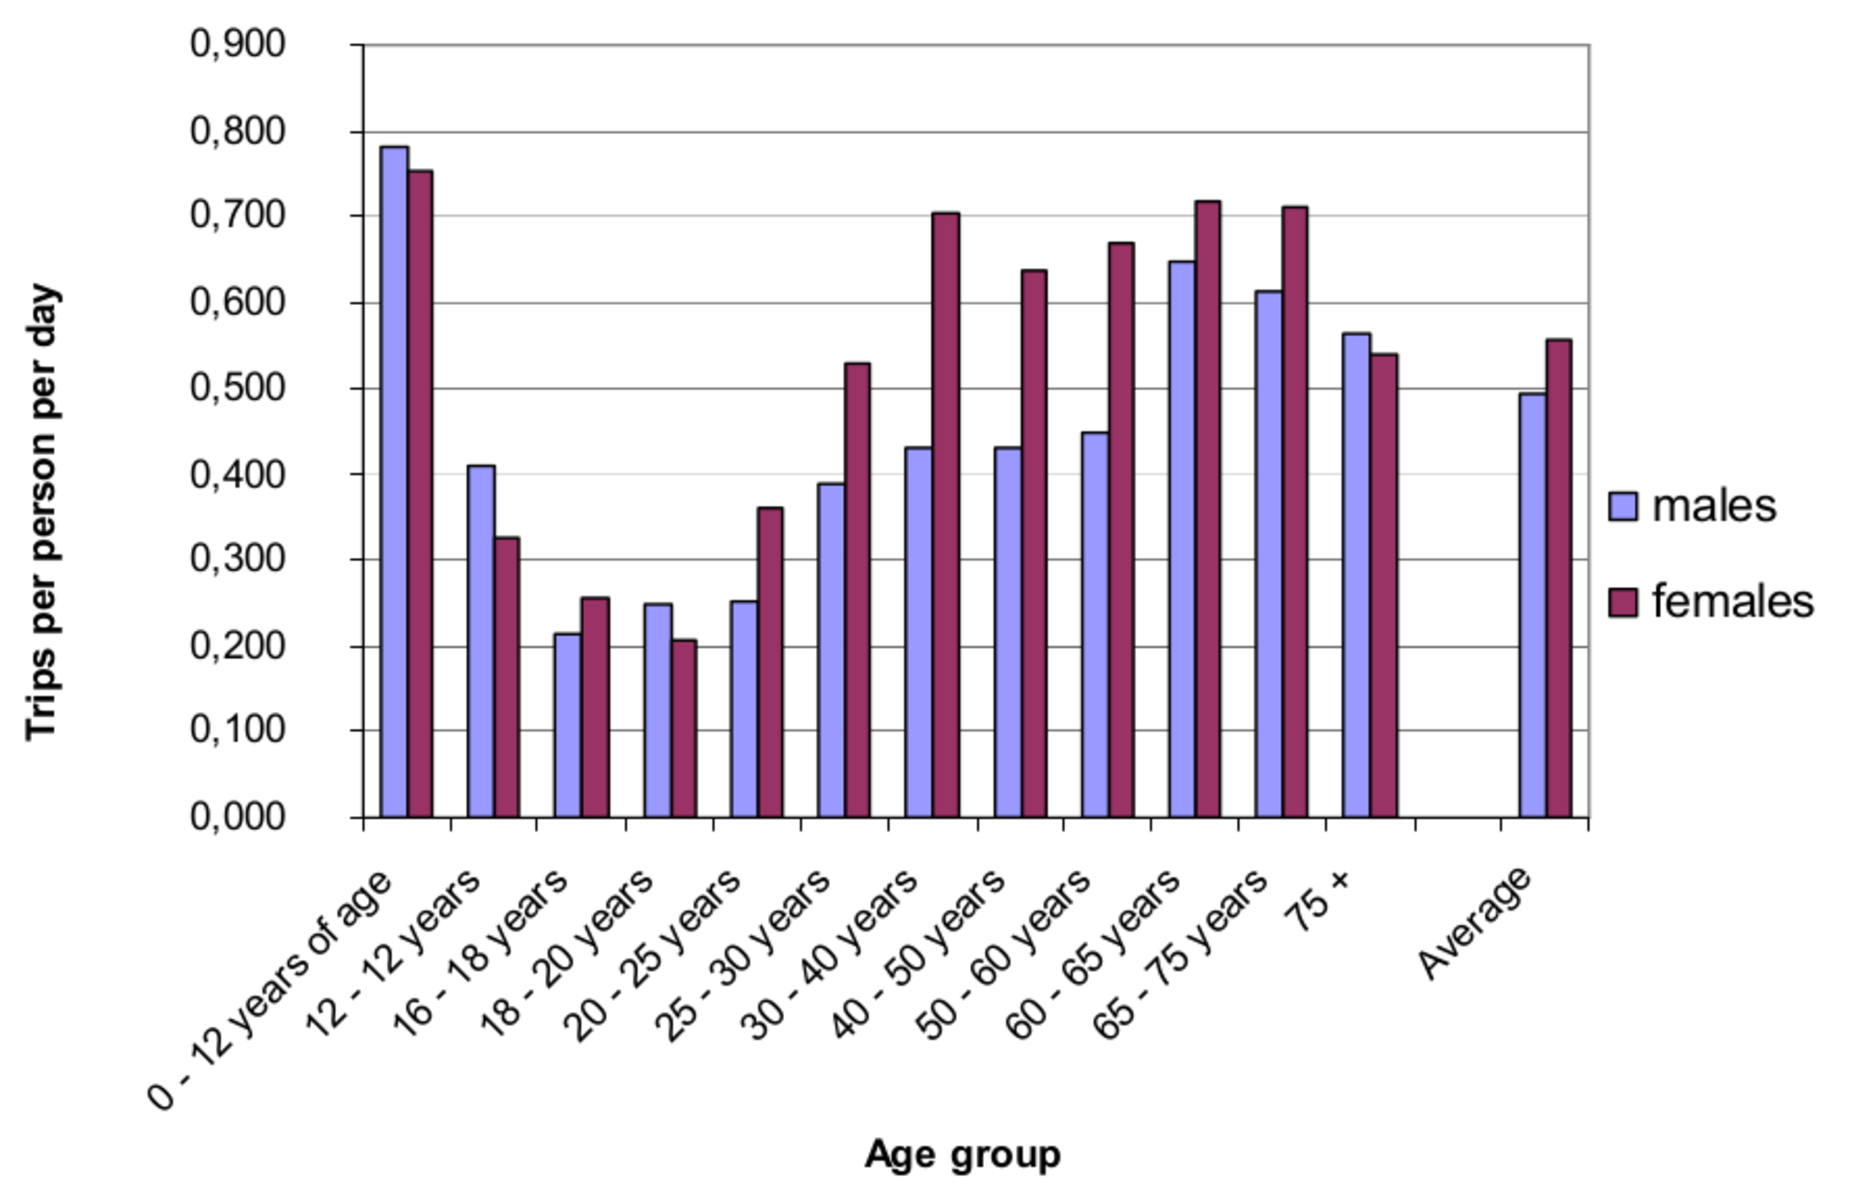
\includegraphics[width=\textwidth]{img/I3_numberOfTripsPerPersonPerDayByAge.pdf}
\centering
\caption[Number of trips per person per day by age group]{
Number of trips per person per day by age group. (NL, 2007 from~\cite{countryReport}) \label{percwalk}}
\end{figure}

In conclusion, outdoor physical activity, particular walking, seems the key role in the maintenance of functional independence at old age.~\cite{Rantakokko2009} By enabling mobility, elderly can keep control of their own life by being able to move outside independently for everyday tasks and social contacts.~\cite{MENSenSTRAAT2014} Walking keeps them fit and healthy and so increases the chance of longer and independent life. Overall, contributing to a better quality of life. 

\subsection{The Rollator}
A lot of elderly use a rollator, or wheeled walker. It helps maintaining mobility and continuing an active lifestyle. It provides stable support and may help avoid falls. Walkers are an important assistant for elderly who face difficulty walking and maintaining balance. The exact amount of rollator users in the Netherlands is unknown. An estimation in 2002 states 160.000 to 300.000 rollator users in the Netherlands~\cite{VeiligheidNL2012} with an average age of 77.7 years according to an article in Trouw.~\cite{Trouw2003} 
For further references we will refer to the wheeled walker as a rollator indicating a hand held walker with four wheels. 


\subsection{Mobility problems}
Getting older means; being less mobile and more fragile.~\cite{VeiligheidNL2012} In general, about 50\% of the pedestrians in the Netherlands have limited mobility abilities and around 10\% of the population has severe difficulties walking and sojourning in the public space.~\cite{Sauter2010} Table~\ref{nrpeople} shows the number of Dutch inhabitants with limited mobility, with the largest group formed by elderly above 65. Also the prediction for 2030 shows an increase in elderly with mobility problems.~\cite{Sauter2010} 

Yearly 18.000 elderly of above 55 need emergency care after a fall on the street. This means that every 30 minutes an elder adult falls so severe that care in the emergency room is needed.~\cite{VeiligheidNL2012} About 2.300 elderly of above 55, need emergency care after a fall with a rollator.~\cite{VeiligheidNL2012} One of the six falls with a rollator is outdoors. (380 falls a year)~\cite{VeiligheidNL2012}

Falls on the street without rollator occur more than falls with a rollator (18.000 to 2.300), but the latter cause more severe injuries. The medical costs for a fall with a rollator are inexplicably higher than a normal fall on the street(table~\ref{costsaccident}). An indication that a fall with a rollator leads to more serious injuries, then a fall with bike or scoot-mobile.~\cite{VeiligheidNL2012}

Fall accidents on the street occur due to behavioural factors (61\%) and environmental factors (58\%). Falls with a rollator can occur because a walker may be difficult to handle, the rollator is unstable or too heavy to handle for the user. A user needs strength and coordination to operate a rollator effectively~\cite{Einbinder2010, Weiss2014}. Environmental influences noted are irregular surface (43\%), obstacles and irregularities (31\%), bad maintenance (16\%) and slippery areas (13\%).~\cite{VeiligheidNL2012} One third of the falls on the street is because an elderly tripped (35\%) over a stone or tile (10\%) or a curb (4\%) and one fifth slipped (20\%) on a slippery surface (12\%).~\cite{VeiligheidNL2012} 

\renewcommand{\arraystretch}{1.5}
% \renewcommand{\tabcolsep}{6pt}

\begin{table}[h]
	\caption[Predicted number of people with limited mobility]{Predicted number of people with limited mobility, Netherlands (Sauter et al. 2010)}
	\label{nrpeople}
	\centering
	\begin{tabular}{|p{63.6pt}|p{44pt}|p{44pt}|p{44pt}|p{44pt}|p{44pt}|p{44pt}|} 
		\hline 
		-& 2005 & 2010 & 2015 & 2020 & 2025 & 2030 \\
		\hline
		Perc of people w limited mobility & 6.1 & 6.3 & 6.7 & 7.0 & 8.2 & 9.4 \\ 
		Number Younger than 65 & 340.000 & 340.000 & 350.000 & 350.000 & 360.000 & 360.000 \\
		Number 65 - 79 & 250.000 & 270.000 & 310.000 & 360.000 & 400.000 & 430.000 \\
		Number 80+ & 410.000 & 430.000 & 460.000 & 490.000 & 660.000 & 830.000 \\
		\hline
		Total number & 990.000 & 1.050.000 & 1.130.000 & 1.200.000 & 1.410.000 & 1.620.000\\
		\hline
	\end{tabular}
\end{table}

\renewcommand{\arraystretch}{1.5}
\renewcommand{\tabcolsep}{0.2cm}
\begin{table}[h]
\caption{Yearly average and total medical costs for 55+, to type of accident. From Letsel Informatie Systeem 2006-2010, VeiligheidNL~\cite{DenHertog2013} \label{costsaccident} }
\centering
\begin{tabular}{|p{236.2pt}|p{70.4pt}|p{70.4pt}|} 
\hline 
& Average costs & Total costs \\
\hline
Private- and traffic accidents on the street & \euro{} 4.500 & \euro{} 220m \\
Fall on the street & \euro{} 4.200 & \euro{} 82m \\
Simplex bicycle accident & \euro{}4.600 & \euro{} 71m \\ 
Rollator & \euro{}12.000 & \euro{} 33m\\ 
Scoot mobile & \euro{} 6.900 & \euro{} 8,9m \\
\hline
\end{tabular}
\end{table}

\subsection{The contribution of the built environment to walkability}
For elderly, who are more vulnerable, environmental attributes can be barriers to an active engagement in urban life. The quality of the immediate environment is a significant determinant of elders well-being, independence and quality of life.~\cite{Vine2012} Because these environmental details are critical for what the older inhabitants can manage in their everyday lives~\cite{Stahl2013, Stahl2008, Clarke2011, Annear2014} creating a walking-friendly environment is important for their independent mobility.~\cite{Sauter2010} The few studies that explore the older inhabitants and pedestrian-ism are arguing that good neighbourhood design can influence physical activity, health and consequently can lead to a longer life time of independence.~\cite{Vine2012, Rantakokko2009, Phillips2013, Beard2009, Rosso2011, Clarke2011}
The environment can have a powerful effect on the amount of walking activity undertaken by older people, thereby influencing their capacity to maintain their well-being and independence~\cite{Vine2012}.

The assessment of a neighbourhood design that supports elderly can be based on walkability. \begin{description}\item[Walkability] is the measure of how friendly the environment is to walking. The extent to which the built environment supports and encourages walking. By being friendly, giving comfort and safety, and provide aesthetic appeal.~\cite{Vine2012, Borst2008}\end{description}
% Vine et al. describes walkability as, the extent to which the built environment supports and encourages walking, by providing pedestrian comfort and safety, with reasonable time and effort and offering visual interest throughout the network. Borst et al. states that walkability is an index of the quality of the neighbourhood. The factors determining it, include, residential density, land-use-mix, street connectivity, aesthetics and safety.

A report from CROW, which is further explained in the next section, about pedestrianism in the Netherlands states that investing in pedestrian policy and making a pedestrian-friendly environment lets the elderly live longer independently.~\cite{Eijnde2011, Crow2014} This means, it requires the environment to provide the best conditions for even the most frail and weak sub-group.

Previous studies have found a relationship between neighbourhood characteristics, physical activity and related health aspects.~\cite{Borst2008} Aspects of the built environment, in particular neighbourhood design, have been found to influence the amount of physical activity undertaken by inhabitants of urban neighbourhoods,~\cite{Borst2008} access to public transport, nearby goods and services, walking for leisure, social interaction and engagement in the community.~\cite{Vine2012} In order to increase the quality of the environment, we need better insight into the influence of the urban design on the walking behaviour of elderly to make it useful for policy and design. 

\section{Problem definition}
\subsection{The forgotten pedestrian in policy}
There is little research carried out on pedestrian satisfaction in the Netherlands. The sparse information about what dissatisfies the pedestrian comes from complaints at local authorities, questionnaires or internet sites. The Pedestrian Quality Needs Project(PQN), identifies what people need for safe mobility in the public space. The project was conducted from November 2006 until November 2010. The main objective was to provide knowledge of pedestrians' quality needs to support walking conditions it the EU. They provide an extensive report on what people require as a pedestrian, and reports stating the current status of pedestrian knowledge in all participating countries.~\cite{Sauter2010} The PQN report of 2010 on walking in the Netherlands states that serious problems and deficits in Dutch pedestrianism are partly or totally hidden from public, scientific and political attention.~\cite{countryReport} They state the following about pedestrian knowledge in the Netherlands: 

\begin{description}
\item[The vicious circle] of no data- no awareness - no priority - no research - no data, needs to be broken.~\cite{Sauter2010, countryReport}
\end{description} 

With specific regard to elderly the PQN report states that large numbers of people already have trouble performing walking and sojourning tasks and because of the ageing of the population these numbers will only increase.~\cite{Sauter2010} Therefore, prevention of falls is important in regard to the safety of pedestrians which is also an age related problem.~\cite{Sauter2010}

The publication about pedestrians in the Netherlands from CROW (2014)~\cite{Crow2014}, states that pedestrians are forgotten in policy and design. CROW is a national knowledge platform for infrastructure, traffic, public transport and public space. A non-profit organisation providing guide-lines for the design, policy and projects with regard to the design of the public space. They state that walking, though one on the main forms of transportation, gets less attention then bicycles, public transport and cars. Pedestrians get more easily forgotten in policy design and maintenance plans. There is a need for a more systematic approach.~\cite{Crow2014} There are two reasons why walking is not part of policy and design plans; first, there is a lack of knowledge about how investments contribute to the tackle of problems. Second, there is no insight how walking can be optimised in policy, design and maintenance plans.~\cite{Crow2014}
With regard to elderly as pedestrians in specific, they state, that a well accessible pedestrian network, and attractive walking routes can contribute to the independence of elderly. Children and elderly are vulnerable in traffic, and elderly pedestrians above 75 have the biggest risk of being victim to traffic accidents with severe endings.~\cite{Crow2014}

MENSenSTRAAT is a network for independent mobility by foot or bike, focussing on the more vulnerable users of the public space. They constructed a pleading call for improving the public space with regard to elderly pedestrians and state that the direct outdoor environment, is crucial for elderly to live independent and stay healthy. Weak sub-groups are often overlooked in the design process and the local governments often forget the importance of street design for the elderly. MENSenSTRAAT states that this needs more attention.~\cite{MENSenSTRAAT2014} 

\subsection{The forgotten pedestrian in research}
Next to the forgotten pedestrian in policy, also little studies can be found on walking behaviour and pedestrians in general~\cite{Vine2012}. A limited number of studies can be found that look specifically at older people's use of the outdoor home environment, how they use it and what problems there are.~\cite{Phillips2013, Stahl2008} Even less studies focus on elderly walking with a rollator outdoors.~\cite{Stahl2008, Stahl2013, Phillips2013} Most studies about elderly, mobility and rollators focus on the interior conditions and accessibility indoors of public buildings, and residences.~\cite{Crow2014, Sauter2010, Verschuur2013} The outdoor environment is significantly important to elderly, but despite this, little research has been conducted on this topic.~\cite{Stahl2008} In addition, little knowledge exists about the factors influencing walking behaviour of elderly. What do elderly perceive as being unpleasant? Moreover, known factors do not always find an integrated place in policy, design and maintenance plans. Let alone, hardly any research can be found that focusses on methods to quantify or map possible problematic factors. 

\subsection{The forgotten pedestrian in data}
Because there is no research on pedestrians there is also no data~\cite{Sauter2010}. The PQN report gives several reasons for this lack of data:
\begin{enumerate}
\item Pedestrians are low on the transport agenda. Lack of sensitivity and political will on collecting data on walking. No counting means no data, no data means no counting.
\item Data that is collected is fragmented and inconsistent. There is a lack of common standards.
\item Indicators and methods for measuring transport are not appropriate for walking.
\item Existing information is not edited for use.
\item Existence of data is not known or hard to access.
\end{enumerate}

Another remark to make is that walking to other forms of transport, multi-modal walking, is almost as extensive as walking from door to door but is often not included in statistics.Therefore, the numbers are often underestimated in the interest of walking when looking at mobility statistics.~\cite{VeiligheidNL2012, Sauter2010} 

As long as the pedestrian is missing in the data, there can be no research and no actions taken to improve policy. While people that have mobility problems, are struck hardest by obstacles in the public space.~\cite{VandeRidder2008} 


\subsection{GIS opportunities}
% Mapping the urban area, to detect problems in order to solve them can be valuable for municipalities and urban planners to improve the situation for elderly and develop focussed interventions.~\cite{Stahl2013} 
% Because the physical aspects of the environment influence walking,~\cite{Leslie2005} 
GIS technologies and databases can provide great potential for studying the environment and neighbourhood characteristics that influences outdoor walkability quality among older people~\cite{Vine2012} and by doing so, fill a bit of the knowledge gap for decentralized governments and urban planners. While the role of geo-data in urban design is recognised nowadays,~\cite{Matthews2003} mapping the environment and the problems with GIS gives more understanding and customized information about the city to its city planners in order to develop new interventions and enhance walkability for rollator users.~\cite{Matthews2003, Svensson2010} GIS is a strong medium to provide urban planners with the data needed to make the urban area friendlier to rollator users and make cost-effective prioritized interventions. It is a rather easy approach to enhance the knowledge about the urban environment, and to locate certain obstacles and flaws that affect accessibility for the impaired citizens.~\cite{Svensson2010} Here we will look at the opportunities that available geo-data in the Netherlands and analysis provides to fill some of the knowledge gaps and make the obstacles for elderly pedestrians more visible. It helps to show that the build environment is often distorted and hostile for the mobile impaired.~\cite{Matthews2003}

\subsection{Lack of detail in (geo) data}
The scarce amount of studies about the elderly pedestrian, stated that more accurate, detailed and up to date data is needed to map walkability indicators for elderly, then the current and accessible geo-data can provide.~\cite{Verschuur2013, Laakso2011} Such detailed data is needed, because every stone counts in regard to frail elderly.~\cite{Matthews2003, Laakso2011} Importance of small details in relation to the larger infrastructure seems needed to map the walking restrictions in the outdoor activity space of elderly with a rollator~\cite{Stahl2008, Stahl2013}. Will GIS be able to map sufficient detail needed for the critical walkability indicators for elderly with a rollator? 

\section{Objective \& Research Questions}
The overall goal of this research is to create awareness of the forgotten pedestrian in policy, research and data. Awareness may trigger possible action at decentralized governments to increase walkability quality and so increase walking activity of elderly people. To keep them fit and healthy, capable to live independently and grow old in their own house and environment. All contributing to less need for healthcare for the growing share of elder population and reduce the cost of elder care.

The specific objective of this research is to analyse and visualize geodata to explore the critical walkability factors for elderly depended on a rollator in the urban outdoor space. The case study is set in Amsterdam, the Netherlands. To achieve this objective, the following research questions will be answered:

\begin{enumerate}
	\item What are the critical walkability factors hindering elderly with a rollator in the outdoor environment?
	\item Which existing geodata can be used to map and analyse these critical walkability factors?
 	\item What geodata can be collected with a smart walker to map and analyse these critical walkability factors? 
	\item How can the available and measured geodata be compared? 
\end{enumerate}

% This research aims at grasping the critical walkability factors that elderly experience while walking outdoors with a rollator and explore the possibilities of geo-data and GIS analysis to map and visualize them. This may increase walking activity of elderly people by raising more awareness and trigger possible action at decentralized governments. Consequently it can support health, the capability to live independently and grow old in their own house and environment. All contributes to less need for healthcare and so reducing costs for elder care. The case study is set in Amsterdam, the Netherlands. 

% The objective is, to analyse geodata of critical walkability factors for elderly people depended on a rollator in the urban outdoor space in favour of supporting outdoors walking activity. 

% % So the overall objective of this research is to analyse the critical walkability factors for elderly people depended on a rollator, in the urban outdoor space. T

% To achieve this objective, the following research questions are developed:

% \begin{enumerate}
% 	\item Investigate the critical factors for walkability in the urban outdoor environment for elderly depended on a rollator.
% 		\begin{enumerate}[a]
% 			\item Literature
% 			\item Experiences of rollator users
% 			\item Local government policy
% 		\end{enumerate}

% 	\item Map and analyse the critical factors by using available geo-data.

% 	\item Map and analyse the critical factors by collected geodata(measuring rollator movements with an accelerometer) and analysis.
	 
% 	\item Compare the available and measured geodata by anomalies in the time series data of speed, slope, and vertical acceleration, using changepoint detection.
% \end{enumerate}


\section{Report Structure}
This report exists of 5 chapters, including this introduction chapter. Figure \ref{reportstruct} illustrates the structure of this report. Chapter 2 describes some background concepts and projects related to this one, which are the inspiration and reference to support this study. Chapter 3 sketches the research area and continues to provide information, per research question, on data, preprocessing and methodology. The final chapter presents the conclusion, the discussion and gives recommendations for future work. Each chapter in this report opens with a short outline of its content.

\begin{figure}[hbp]
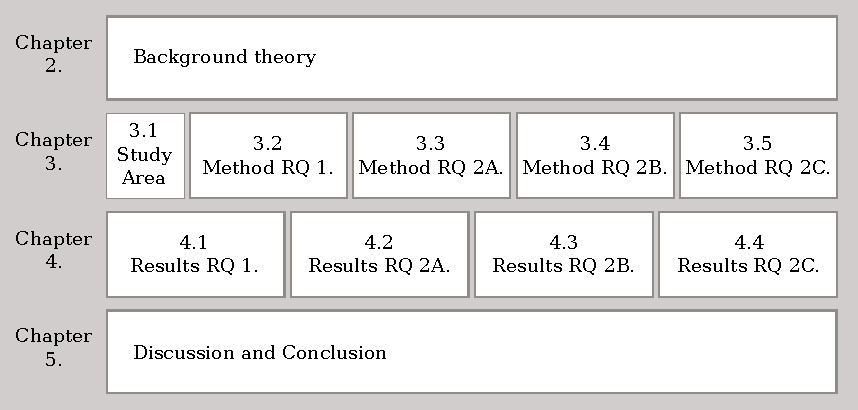
\includegraphics[width=\textwidth]{img/I4_ReportStructure.pdf}
\centering
\caption{Report Structure}\label{reportstruct}
\end{figure}
